%!TEX root = ../thesis.tex

\chapter{Introduction}

\ifpdf
    \graphicspath{{Chapters/Figs/Raster/}{Chapters/Figs/PDF/}{Chapters/Figs/}}
\else
    \graphicspath{{Chapters/Figs/Vector/}{Chapters/Figs/}}
\fi


%********************************** % Section  **************************************
\section{Embedded Systems}
Information processing and computer usually refer to Personal-Computers. However, according to several forecasts, the future of information and communication technologies (ICT) is characterized by terms such as \emph{ubiquitous computing}, \emph{pervasive computing}, \emph{ambient intelligence} and the \emph{post-PC era}. These terms reflect the fact that computing (and communication) will be everywhere, the information available anytime and anywhere. The technology leading this future is the embedded systems technology.%The main technology needed for next-generation ICT systems are the \textbf{embedded systems}.
\par Embedded systems, which are part of the broader area of Cyber-physical systems (CPS), are special-purpose computer systems designed to control or support the operation of a larger technical system, see \cite{BerkleyCPS} for a conceptual map. Unlike the general-purpose computer, they only perform a few specific and more or less complex pre-defined tasks. The typical use cases of CPSs are medical devices, aerospace, autonomous systems (like robots, autonomous cars or Unmanned Aerial Vehicles - UAVs), agriculture and buildings. CPS interact with the physical world and must operate dependably, safely, securely, and efficiently and in real-time.
\par In a simpler case, software consists of a single program running in a loop, starting at power-on, and responding to certain internal or external events. In more complex cases (robotics or aerospace) operating systems are employed providing features like multitasking, synchronization, resource management, among others.

\paragraph{}There are almost no areas of modern technology in which we could do without embedded systems. Rajkumar et al. \cite{Raj10} described CPS as \emph{the next computing revolution}. CPSs are starting to pervade areas such as wearable electronics and domotic applications. As they are becoming ubiquitous, we are gradually do not notice them anymore. Contemporary cars, for example, contain around 60 embedded computers\footnote{according to a 2014 report from the Alliance of Automobile Manufacturers}. The driver is not aware of them but is utilizing their functionality.

\paragraph{}By definition, embedded systems operate in real-time domains, which means that their temporal behavior is equally important as their functional behavior. While formal methods are quite mature for verifying functional properties of the model, the methods for proving that temporal behavior is not yet mature and can be used only to show that particular states are never reached. Therefore, verifications is usually based on testing and the quality of such tests depends mainly on the experience and intuition of the designer. 


%********************************** % Section  **************************************
\section{Mixed-Criticality}
%As a consequence of the increasing complexity of control algorithms, 
As a consequence of the evolution of integrated systems, to achieve better flexibility, and for economic reasons, embedded systems are being used into more safety-critical areas. 
%Generally the integrity of the whole system depends on them and any failure could have severe consequences: for example endanger human safety.
This means that they integrate multiple functionalities (tasks) with different safety-critical levels, such as flight-critical and mission-critical tasks, on a single, shared hardware device. Criticality can include all forms of dependability (availability, integrity, etc.) \cite{dependability}, but it usually refers to functional safety, i.e., the absence of catastrophic consequences on the user and the environment. %The concept of criticality depends on the application, such as navigation or braking. 
% Example of critical something

\paragraph{}A more formal definition of criticality can be obtained with reference to the safety standards (see \cite{MCSmisconception} for a more detailed discussion) that define the design and development processes for safety-critical embedded systems (hardware and software). There are a variety of domain specific safety standards, such ISO 26262 for road vehicles. This work is focused on aerospace where is usual to refer to DO-178C \cite{do178c} for avionic software and ARINC 653 \cite{arinc653} for avionics real-time operating systems. %DO254 for avionic hardware
\begin{description}
	\item[DO-178C] (aka EUROCAE-ED-12B) was drafted by a co-operation of the European Organization for Civil Aviation Equipment (EUROCAE) and its US counterpart. The standard considers the entire software life-cycle and provides a basis for avionic systems certification. It defines five levels of criticality, from A (components whose failure would cause a catastrophic failure of the aircraft) to E (components whose failure have no effect on the aircraft or pilot workload) as in table \ref{tab:DAL}. This is the primary document by which the certification authorities approve all commercial software-based aerospace systems.
	\item[ARINC-653] is a software specification for space and time partitioning in safety-critical avionics real-time operating systems. It allows the hosting of multiple applications of different software insurance levels (SIL) on the same hardware in the context of an Integrated Modular Avionics (IMA) architecture. Each software component is inside a partition and has its memory space and dedicated time slot. The current work includes the enhancement of ARINC-653 for multi-core processor architectures.
\end{description}
All these documents are used by the certification authorities that must establish system safety. In this process, developers need to convince official entities that all relevant hazards have been identified and dealt with. In general, they are very reluctant (or even refuse) to approve safety-related technical systems with non-trivial complexity (like multi-core platforms). The reason lies mainly in a lack of confidence in such complex systems, and in the considerable effort needed for their verification. %Validation answer the question "Am I building the right system?", verification answer "Am I building the system right?" (both are needed in reality)

\begin{table}
\begin{center}
\begin{tabular}{cll}  
\toprule
Level & Failure Condition  & Failure Rate \\
\midrule
A & Catastrophic & $10^{-9}$/h \\
B & Hazardous 	 & $10^{-7}$/h \\
C & Major 		 & $10^{-5}$/h \\
D & Minor 		 & $10^{-3}$/h \\
E & No Effect 	 & N/A \\
\bottomrule
\end{tabular}
\caption {Failure rate per DO-178C criticality level}
\label{tab:DAL}
\end{center}
\end{table}

\paragraph{} All standards define different levels of concerns, in the aerospace field they are called Safety Integrity Level (SIL) in IEC 61508 and ARINC 653, or Design Assurance Level (DAL) in DO-178C. The levels indicate the severity and frequency of a function failure and assign requirements to failure probability, architectures, and design processes to each of the levels. They also regulate the combination of functions with different levels; so, they provide a basis for Mixed-Criticality systems design.
\par Because larger systems, such as vehicles or aircrafts, include a few safety-relevant applications and many non-critical ones, such as air conditioning or infotainment, mixed criticality is a well-known problem for both research and industrial actors. Safety standards strongly regulate mixed-critical design and integration. The generic standard IEC 61508 requires that \emph{sufficient independence} is demonstrated between functions of different criticalities. We can design the system as only high-critical, this approach is usually too costly and can even lead to non-functional implementation. Since designing with the more stringent process requirements of safety-critical functions and also non-critical functions, which are often third party provided (e.g., infotainment), is far too costly, \emph{sufficient independence} is the only viable option. 

%\paragraph{} The determination of the criticality is, in general, the result of the evaluation of the possible consequences of a failure (severity or hazard) on the occurrence of a failure.

\subsection{Robust Partitioning} 
The concept of \emph{Robust partitioning} is defined differently in standards which make it complicated to extract the official definition \cite{robustpartitioning}. Rushby \cite{goldenrule} defines the \emph{Gold Standard for Partitioning} as \emph{"A robustly partitioned system ensures a fault containment level equivalent to its functionally equivalent federated system."}. Federated architecture is the traditional design for avionic architecture where each application is implemented in self-contained units. Wilding et al.\cite{goldenruleinvariant} define the \emph{Alternative Gold Standard for Partitioning} as \emph{"The behavior and performance of software in one partition must be unaffected by the software in other partitions"}, which is a stronger property and a sufficient condition to establish robust partitioning. In any case, robust partitioning consists of the following the concepts:
\begin{itemize}
\item \emph{Fault Containment}. Functions should be separated in such a way that no failure in one application can cause another function to fail. Low criticality tasks should not affect high criticality tasks.
\item \emph{Space Partitioning}. No function may access the memory space of other functions (unless explicitly configured).
\item \emph{Temporal Partitioning}. A function's access to a set of hardware resources during a period of time is guaranteed.
\end{itemize}

\paragraph{} ARINC-653 contains its interpretation of robust partitioning: \emph{"The objective of Robust Partitioning is to provide the same level of functional isolation as a federated implementation."}. This space partitioning concept can be implemented on multi-core systems with the help of the Real-Time Operating Systems.

\subsection{Operating systems for Mixed-Criticality applications}
The core concept of demonstrating sufficient independence among different function can be approached using Kernels and schedulers that guarantee resource management to provide independence in the functional and time domain; separation kernels are the most notable example.
\par A separation kernel is an operating system-level resource manager that enforces \emph{spatial and temporal separation} among functionalities or partitions that are managed by it. First proposed by John Rushby in 1981 \cite{separationkernel}, according to him \emph{"the task of a separation kernel is to create an environment which is indistinguishable from that provided by a physically distributed system: it must appear as if each regime is a separate, isolated machine and that information can only flow from one machine to another along known external communication lines. One of the properties we must prove of a separation kernel, therefore, is that there are no channels for information flow between regimes other than those explicitly provided."}. In another word a single board platform that is indistinguishable by a federated system. 
\par A typical structure of a separation kernel is depicted in figure \ref{fig:separationkernel}. 
\begin{figure}[htbp] 
\centering    
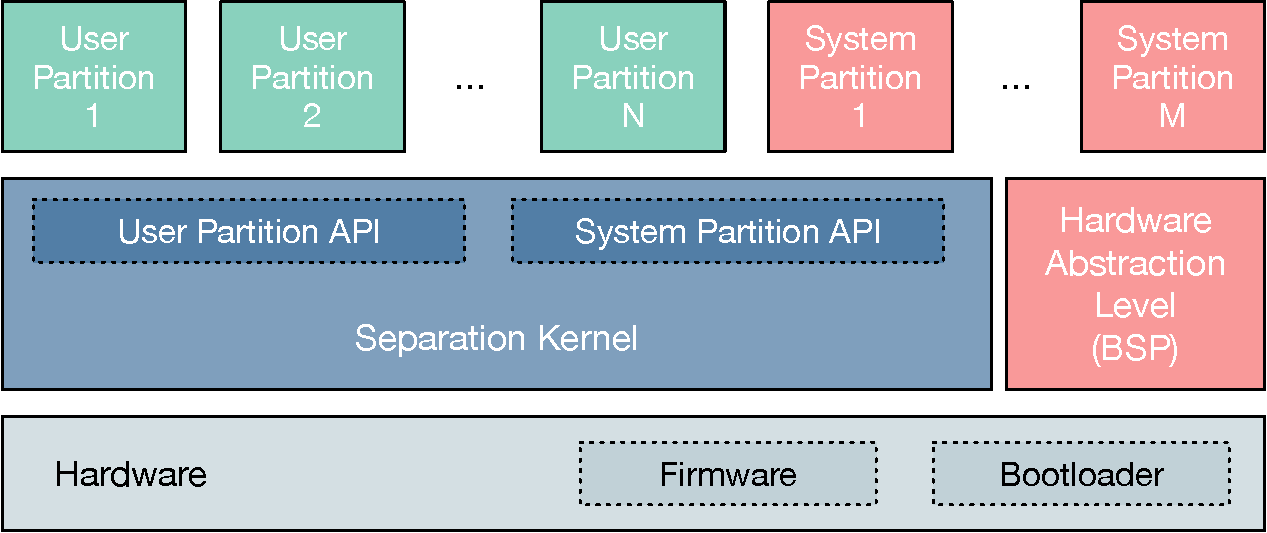
\includegraphics[width=0.7\textwidth]{SeparationKernel}
\caption{Typical Separation Kernel Architecture}
\label{fig:separationkernel}
\end{figure}
A partition is a logic unit maintained by the separation kernel, and each of them is separated from the other. For each partition, the separation kernel provides resources such as physical memory space, I/O memory space, CPUs, and so on (spatial separation). Moreover, separation kernels are typically implemented using time-triggered schedulers and assigning each partition a dedicated time slot in a cycle to provide time separation. Usually two type of partitions are supported: \emph{User Partitions} and \emph{System Partitions}. The partitions are identified configured by the system designer, which is a trusted person. The content of a user partition does not need to be approved by the designer and can be arbitrary, even malicious \cite{mils}, whereas a system partition contains applications and data supplied and approved by the designer. All partitions use the API (Application Program Interface) provided by the separation kernel to interact with it. Since partition are spatially isolated they cannot communicate each other, through the kernel API, they can communicate under the supervision of the kernel. This communication occurs via communication object that is statically configured by the designer. The separation kernel also provides the \emph{Hardware Abstraction Level} called \emph{Board Support Package} (BSP). It contains a set of drivers for specific hardware components, and it is approved by the designer. Since it provides an abstraction of the underlying hardware, an onboard support package can be exchanged without changing the content of any partition.

\paragraph{} Separation kernels are gaining importance thanks to the increasing needs of adoption of multi-core embedded systems.


%********************************** % Section **************************************
\section{Multi-core embedded systems}
The traditional approaches to provide more processing bandwidth were to increase the CPU clock frequency, increase the instruction level parallelism through instruction pipelines, increase the cache size and number of cache levels and so on. With today's technology, this approach is no longer sustainable. Increasing CPU frequency causes excessive power consumption and thermal dissipation loss and raises more and more problems due to internal chip design. Parallelization has become a key solution for this problem. For this reason multi-core platforms have the potential to meet these requirements by offering greater computational capabilities and advantages in size, weight, and power (SWaP). 

\paragraph{} However, in a multicore system different cores share hardware resources such as caches and central memory, which were developed focusing on maximizing the overall performance, but when placed in the safety-critical context introduce challenges to predictability.
\par Safety-critical multi-core CPS are still not fully embraced by industry for safety critical applications. For example, aerospace systems are subject to costly and time-consuming certification processes, which require a predictable behavior under fault-free and certain hazardous conditions, hard to prove in multi-core platforms. Albeit the industry is moving towards higher exploitation of commercial-off-the-shelf (COTS) devices to reduce development cost\cite{mulcors}, as well as exploiting the low SWaP characteristics of multi-core, despite the fact that the use of such boards is challenging for certification.

\paragraph{} The introduction of COTS multi-core processors is by motivated several aspects:
\begin{itemize}
\item Provide a long-term answer to the increasing demand of processing power.
\begin{itemize}
\item Increased performance: better exploitation of the thread parallelism
\item Increased integration: Less equipment to perform the same functionality or same equipment to
host more functionality
\item Reduce environmental footprint: Fewer embedded equipment, less power consumption, less dissipation compared to
the single core equivalent
\end{itemize}
\item Anticipate mass market obsolescence of single-core processors.
\item Be able to "simplify” the overall system architecture (for example a partitioned architecture can avoid Ethernet communication).
\end{itemize}

\paragraph{} The barrier to the adoption of the multi-core technology is its complexity of the certification. For the certification process it is important to ensure the \emph{Execution Integrity} of its software components. That means it will be correctly executed in a nominal situation, and the system state will be predictable in non-nominal situations (internal faults). Moreover, it must be possible to perform a \emph{WCET analysis} (Worst Case Execution Time) of the embedded software. Timing information is tightly coupled with both software and hardware architecture since they introduce \emph{interferences} between parallel applications that are reflected in timing delays. In COTS this analysis become even more difficult because of the lack of documentation on the system design.

\subsection{Hardware interference channels} 
Applications running on different cores of a multi-core processor are not executing independently from each other. Even if there is no explicit data or control flow between these applications, a coupling exists at platform level since they are implicitly sharing platform resources. A platform property which may cause interference between independent applications is called a hardware interference channel. The analysis of hardware interference channels requires a deep understanding of the platform architecture including the CPU internals.
\par In this work, we consider only commercial multi-core platforms rather than designing new architectures. Therefore we assume that the platform implements the Unified Memory Model, which means that all cores share the same physical address space. Figure \ref{fig:unifiedmemorymodel} depict a typical architecture of such platform.

\begin{figure}[htbp] 
\centering    
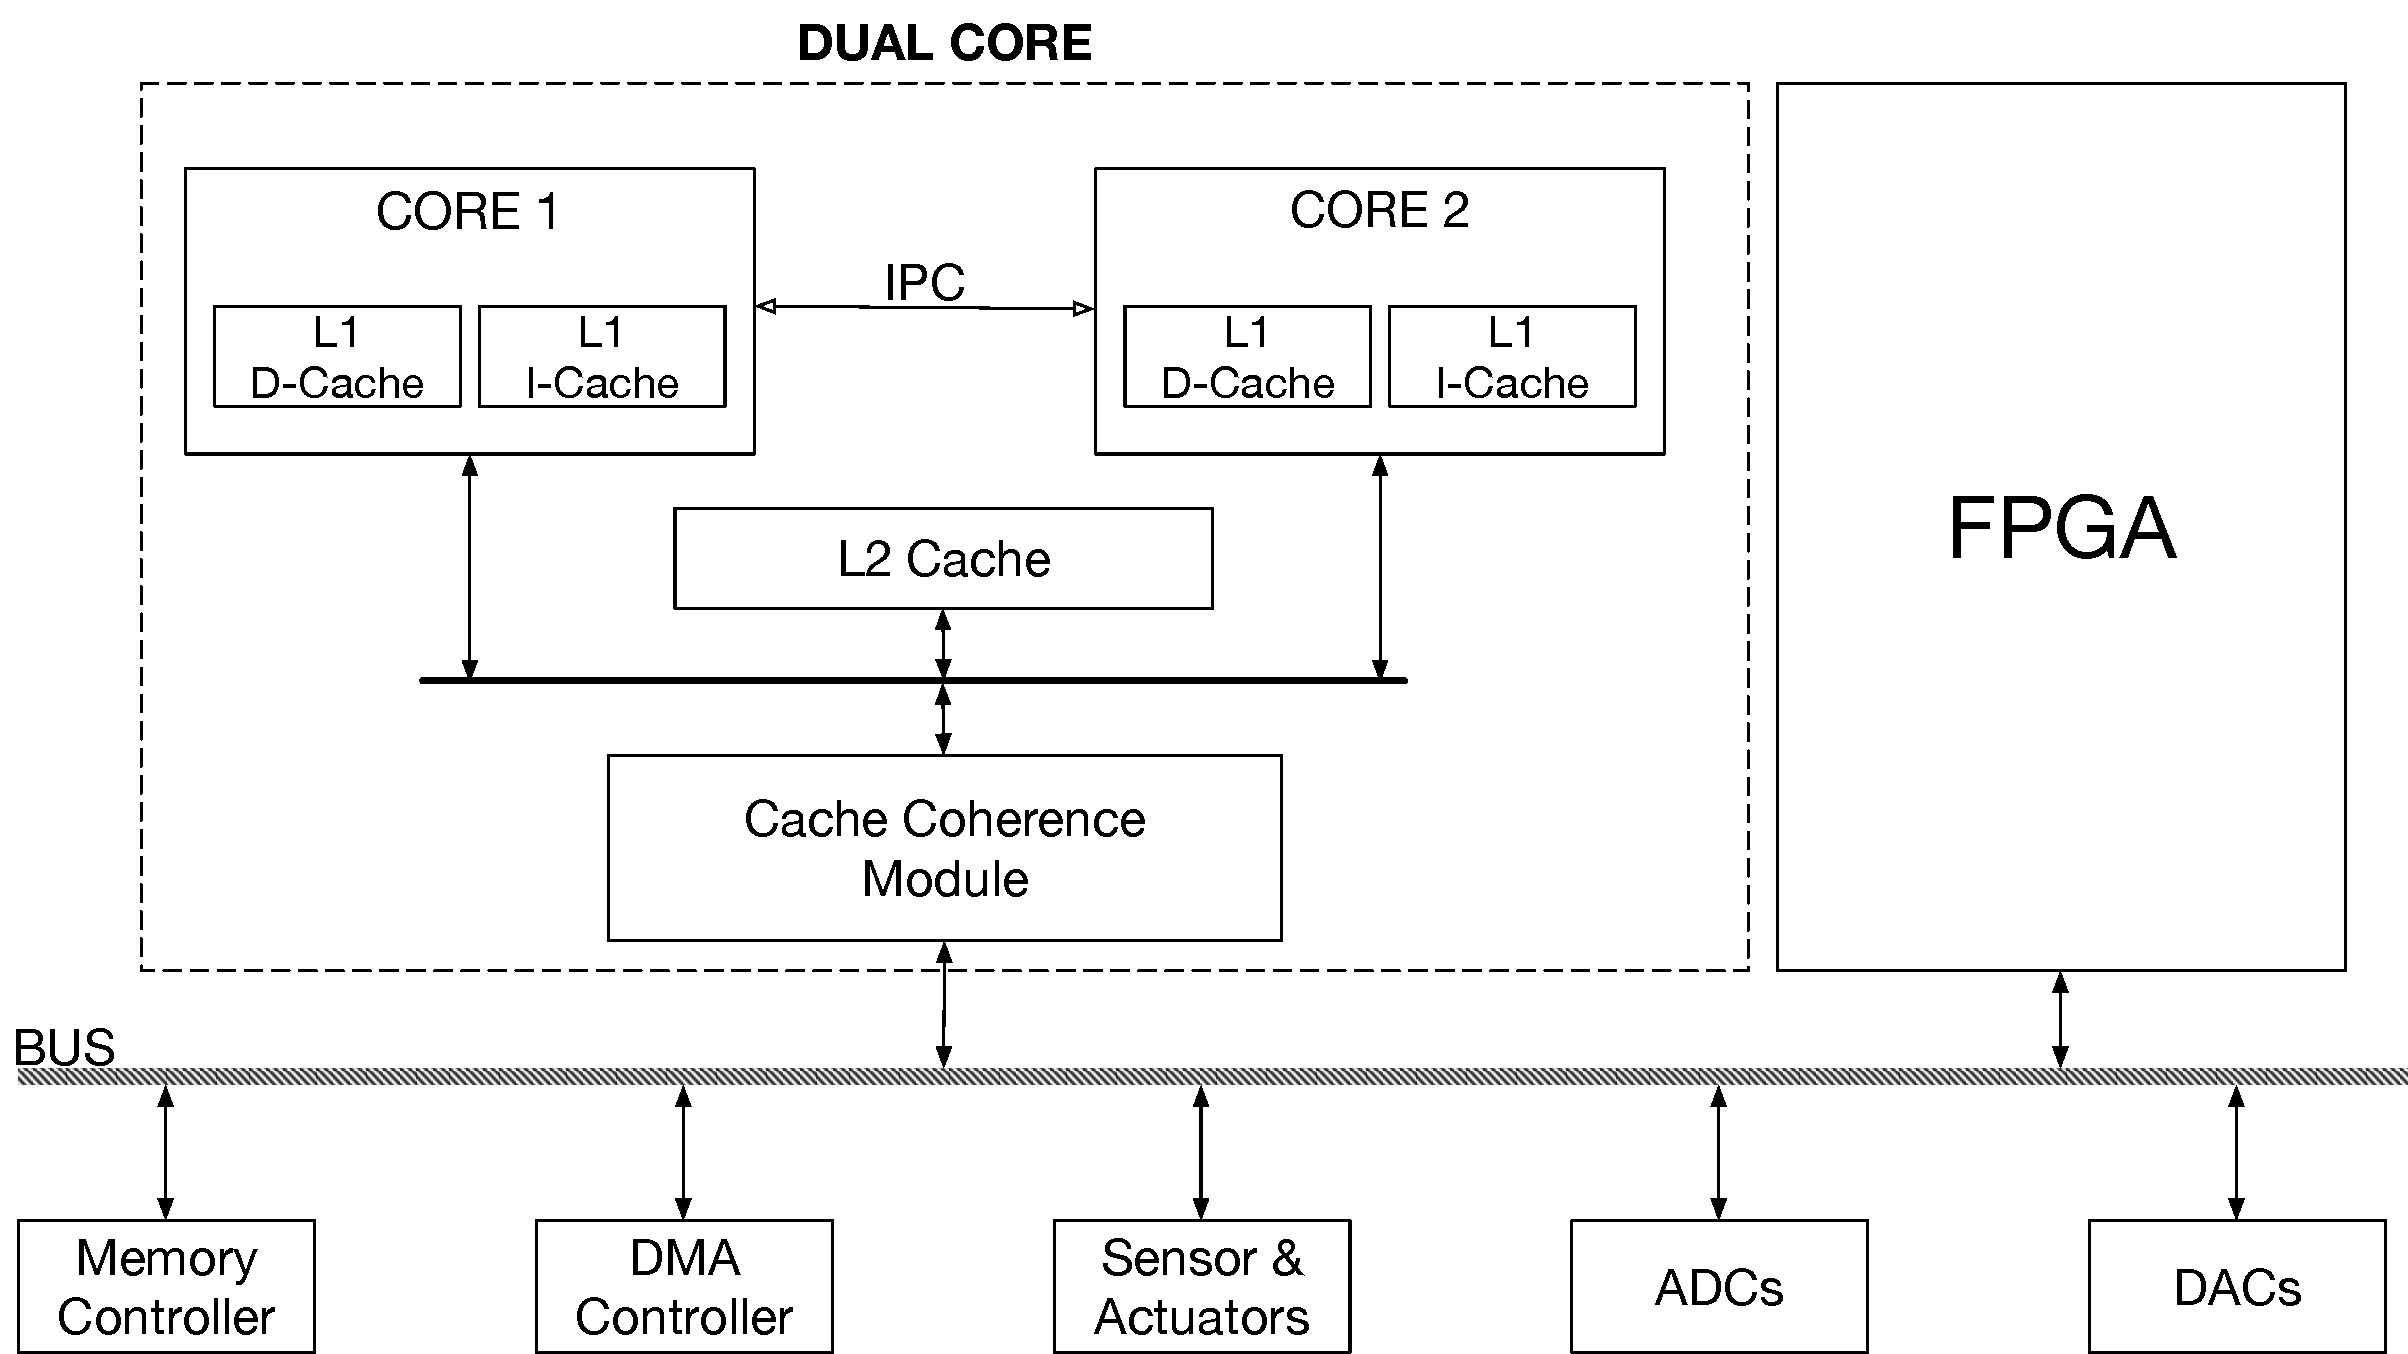
\includegraphics[width=1.0\textwidth]{UnifiedMemoryModel}
\caption{Unified Memory Model Architecture}
\label{fig:unifiedmemorymodel}
\end{figure}

\subsubsection{Caches}
While two different cores can execute independently as long as they are not using shared resources, caches may introduce cross-CPU interference trough \emph{Cache Coherency} and \emph{Cache Sharing}. The L1 cache is typically divided into data and instruction cache while all other levels store data as well as instructions. Most multi-core processors have a dedicated L1 data and instruction cache for each core while other levels might be shared or not depending on the architecture. Shared caches are an essential cause of interference in a multi-core processor. If data used by tasks are small enough to fit inside the private cache of the processor no performance loss occur, if it is not the case, data are replaced according to some \emph{cache replacement algorithm} on demand of executing tasks among all cores. Therefore tasks start to experience long delays due to the recurring access to memory.

%\subsubsection{Cache Coherency}
\paragraph{} Another important aspect related to the use of caches is the consistency of local caches connected to a shared resource. Cache coherency is crucial in multi-core systems because: if one of the local caches of a core contains a reference to a physical resource, and the cached value is more recent than the value stored in the physical resource itself then any read access from any core must provide the value cached. In multi-core processors, cache coherency is solved by utilizing the core communication bus. So this mechanism determines how the memory system transfers data between processors, caches, and memory.

\subsubsection{Interconnect}
Multi-core processors are often part of a System on Chip (SoC) where the cores are packed together with peripherals such as external memory, serial I/O and Ethernet. To handle all requests to the shared peripherals, an \emph{interconnect} is implemented to arbitrate the requests. It is the key point where all the accesses are performed. Indeed, the interconnect has been built to sustain a higher bandwidth to serve all cores efficiently. Usually, a significant source of performance degradation is the concurrent access to shared Bus and shared I/O device such as the graphical device, the GPIO (General Purpose Input Output) or the network interface. If a device can handle one request at a time, it may block the second request for hundreds of microseconds, or even worst to milliseconds. Moreover, shared devices can also rise Interrupts. On multi-core platforms, a hardware interrupt is typically routed to one core. If multiple devices are attached to one interrupt line and the devices are not served by the same core, the core which receives the interrupt must pass this interrupt also to the other core(s). All these factors worsen the determinism of the systems and WCET analysis. Indeed, the execution time of software on one core depends on software executed on the other cores because of potential inter-core conflicts. The internal workings of the interconnect and how it prioritizes the requests are often part of the manufacturer's intellectual property, and they heavily impact on the amount and the duration of interferences. It may be difficult to determine an upper bound on their impact whatever the concurrent software even with full information on the design.
\par Characterizing the behavior of the interconnect in every possible situation in multi-core COTS is technically difficult. To overcome this problem the \emph{Interconnect Usage Domain} can be defined as a set of constraints restricting the accesses to the interconnect. The usage domains give the possibility to treat the interconnect as black-box. The objective is to reach an acceptable characterization of the interconnect behavior to enable further analyses even with poor documentation on the behavior.

\paragraph{} How these interference channels impact of the concurrent application also depends on the software architecture.

%\subsection{Software Interference}
%Obviously tasks interfere with each other due to access to shared I/O devices. However, can be noticed that the Operating Systems can be source of interference too. It must provide an execution environment for the hosted applications which on the one hand hides the platform characteristics from the hosted applications and on the other hand strictly controls the use of platform resources for all applications. Usually the operating system uses some additional software components called Board Support Package (BSP), it is the implementation of specific support code for a given board that conforms to a given operating system.   
%\par The diversity of Multi-Core System on Chip (MPSoC) architecture leads to additional effort (and issues) during certification since the operating systems, the BSP and the code on top of them, must be certified by authorities. 

\subsection{Parallelism basic concepts}
There are several types of parallelism used in multi-core programming, we can fist distinguish between \emph{Task Level Parallelism}, \emph{Data Level Parallelism}, and \emph{Instruction Level Parallelism} \cite{computerarchitecture}. Instruction level parallelism refer to overlapping the execution of instructions to improve performance. There are two largely separable approaches to exploiting this parallelism approach: \begin{enumerate*} \item an approach that relies on hardware to discover and exploit the parallelism dynamically, and \item an approach that relies on software technology to find parallelism statically at compile time.\end{enumerate*} Data level parallelism focuses on distributing the data across different cores, which operate on the data in parallel. It is commonly applied on regular data structures like arrays and matrices by working on each element in parallel. Finally, Task level parallelism focuses on distributing tasks (functional units) across cores. While Instruction and Data Level Parallelism are highly exploitable in FPGA and GPU, in this work we focus only on Task Level Parallelism.
\paragraph{} At system level, Task Level Parallelism can distinguished into two other classification: \emph{Asymmetric Multiprocessing} (AMP) and \emph{Symmetric Multiprocessing} (SMP).

\subsubsection{Asymmetric Multiprocessing}
In this approach each core runs its own single-core aware application (a partition) as in figure \ref{fig:AMP}. Therefore, scheduling inside a partition is sequential. The advantages of using this programming approach are:
\begin{itemize}
\item applications do not need to be multi-core aware; this simplifies the design.
\item reduced need to mutual exclusion.
\item interferences are mainly caused by shared caches, memory, I/O buses and concurrent access to shared devices.
\end{itemize}
The disadvantages are:
\begin{itemize}
\item all applications must be certified to the highest assurance level since they have full access to the processor;
\item it can be hard to identify different single-core aware, independent applications; this can limit the use of cores to few of them;
\item synchronization among applications running on different cores is more complex.
\end{itemize}

\begin{figure}[htbp]
  \centering
  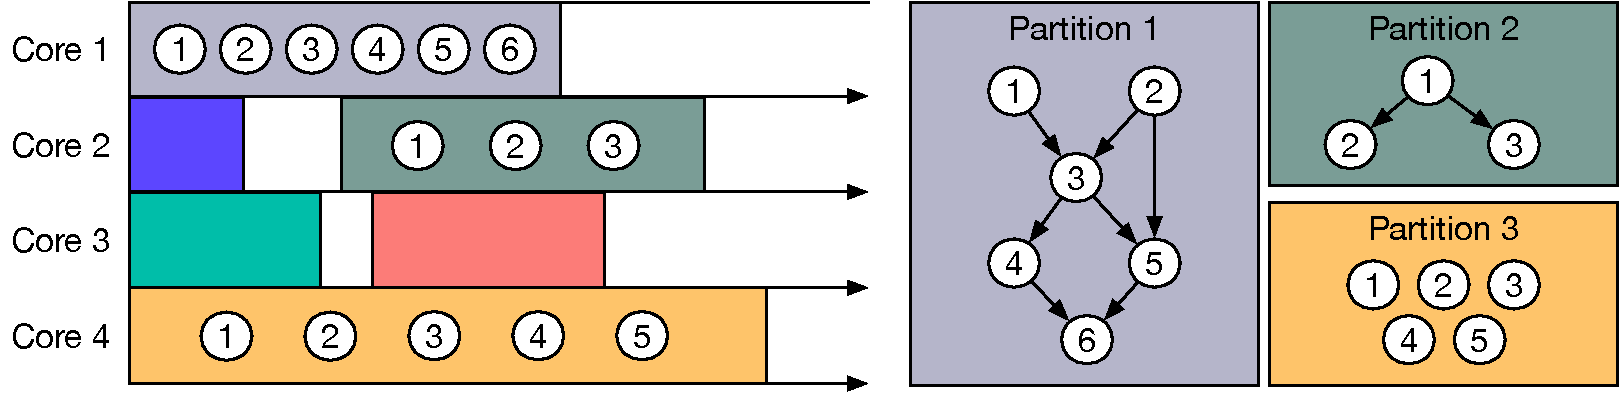
\includegraphics[width=0.7\textwidth]{AMP}
  \caption{Example of Asymmetric Multiprocessing}
  \label{fig:AMP}
\end{figure}

\subsubsection{Symmetric Multiprocessing}
In this approach each application has access of all cores. Threads inside the partition run concurrently and the Operating System typically controls cores and platform resources as shown in figure \ref{fig:SMP}. The advantages of this approach are:
\begin{itemize}
\item More flexibility is allowed and better load balancing can be achieved.
\item There is only one system component responsible for the partitioning.
\item Different safety-levels are allowed in the system (mixed-critical systems).
\item Application can still be completely isolated by the other, e.g. by disabling concurrent execution.
\item Inter-process conflicts does not impact time and space partitioning as they occur inside the same partition.
\end{itemize}
\par The disadvantages comes from this additional system level software components:
\begin{itemize}
\item System level components responsible for the partitioning are complex and must be certified with the highest level of insurance.
\item Synchronization effort can be higher.
\item Due to the shared system software layer, an implicit coupling of unrelated threads cannot be completely avoided.
\end{itemize}
A careful design can limit the impact of these drawbacks. 

\begin{figure}[htbp]
  \centering
  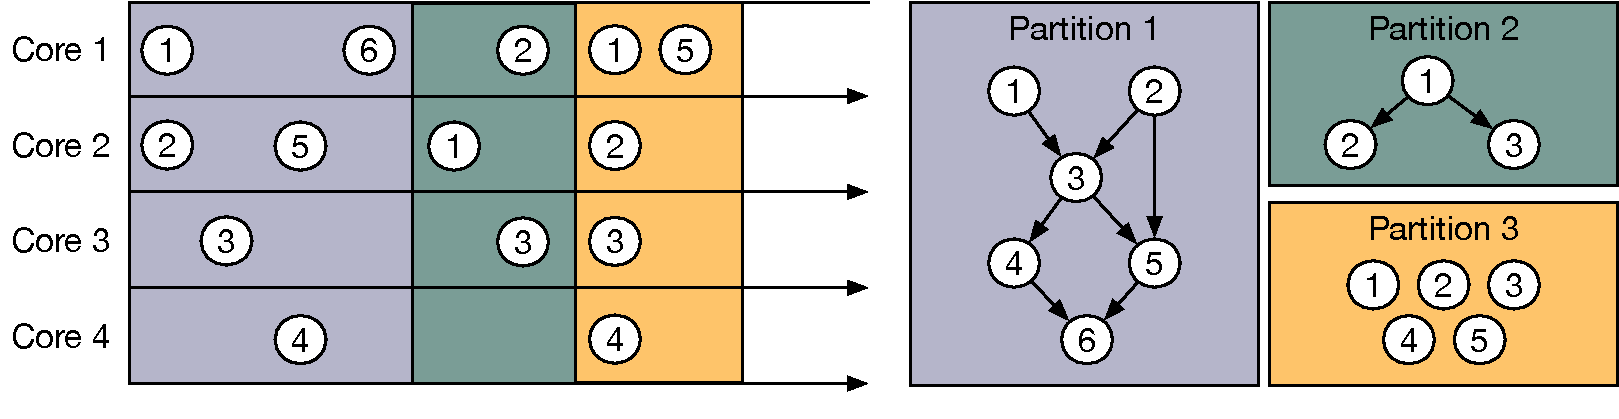
\includegraphics[width=0.7\textwidth]{SMP}
  \caption{Example of Symmetric Multiprocessing}
  \label{fig:SMP}
\end{figure}

\subsubsection{Selected approach}
The asymmetrical approach presents some difficulties in the demonstration of robust partitioning. It is interesting for very specialized applications, for example where, in a dual-core platform, one core is completely dedicated to I/O processing and the other core runs the application software. On the other hand, the symmetric approach needs to be considered to take benefit from platform. All its drawbacks  are manageable if the systems runs under control of the (trusted) operating systems and the design take into account all the possible issues. Moreover we assume that future embedded systems have to host, besides the critical applications, an increasing number applications with high performance requirements but lower criticality.

\paragraph{} Implementing a mechanism to isolate different application inside a multi-core platform is crucial. A virtualization layer hosting several virtual machines can provide this service.

%********************************** % Section  **************************************
\section{Virtualization in Embedded Systems}
The main concept for the design of a mixed-critical system is, first and foremost, the demonstration of sufficient independence among software components. System virtualization, which is the abstraction and management of system resources, facilitate the integration of mixed-criticality systems \cite{multipartes}. This approach results in independent virtual machines that are fully contained in an execution environment that can not affect the remaining system. 

\subsection{Overview}
Platform virtualization refers to the creation of \emph{Virtual Machines} (VMs), also called guest OS, running on the physical machine and managed by a \emph{hypervisor}. Virtualization technology enables concurrent execution of multiple VMs on the same hardware (single or multi-core) processor. Virtualization technology has been widely applied in the enterprise and cloud computing field, however, in recent years, it has been increasingly deployed in the embedded systems domain. Virtualization for embedded systems must address real-time behavior, safety, and security such that it offers protection against external attacks and unintended
interactions between the critical and non-critical components of the system. The hypervisor provides an isolation mechanism that can encapsulate an entire OS and applications into a Virtual Machine (VM).

\subsection{Hypervisor types}
In 1974 Gerald J. Popek and Robert P. Goldberg \cite{popek1974formal} classified hypervisors in two categories:
\begin{itemize}
\item \emph{Level II hypervisor} is software layer that runs on top of a General Purpose Operating System (GPOS) \cite{Kleidermacher2013} (fig. \ref{fig:HypervisorL2}). It takes advantage of the underlying Operating System services and hardware abstraction to enable the creation of virtual machines. However, the security of type II hypervisors is as robust as the host GPOS. Therefore, the hypervisor can be subverted by one of the security gaps in the host GPOS, thereby corrupting the entire system. Additionally, the host OS layer increases system complexity and overall code size, which is a major factor for resource-constrained embedded systems. As a result, type II hypervisors are not suited for most embedded systems.
\item \emph{Level I hypervisor} is software layer that runs directly on the hardware platform (bare-metal) (fig. \ref{fig:HypervisorL1}. This approach avoids the complexity and inefficiency of GPOS, and can achieve a higher level of isolation for safety and security critical applications \cite{Kleidermacher2013}.
\end{itemize}

\begin{figure}
  \begin{subfigure}{0.5\textwidth}
    \centering
    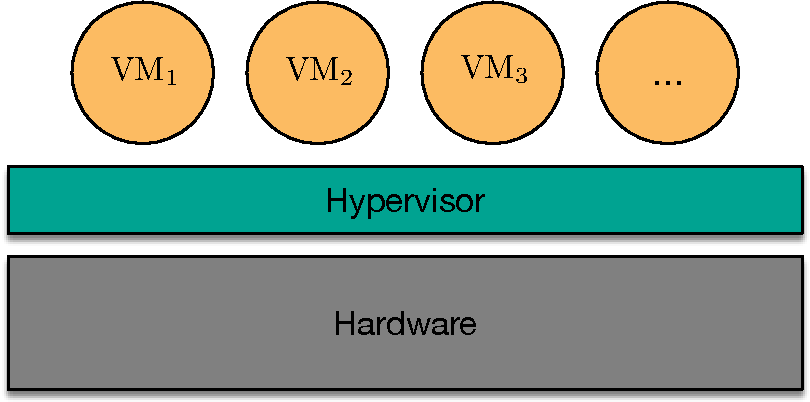
\includegraphics[width=.9\textwidth]{HypervisorL1}
    \caption{Type I}
    \label{fig:HypervisorL1}
  \end{subfigure}%
  \begin{subfigure}{0.5\textwidth}
    \begin{subfigure}{\textwidth}
      \centering
      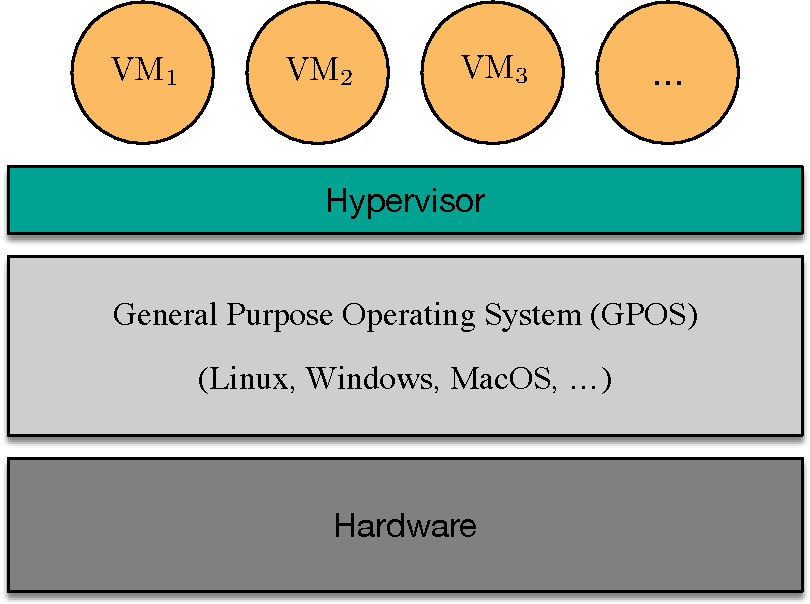
\includegraphics[width=.8\textwidth]{HypervisorL2}
      \caption{Type II}
      \label{fig:HypervisorL2}
    \end{subfigure}
  \end{subfigure}
  \caption{Hypervisor Types}
  \label{fig:interactions}
\end{figure}
The selected operating system, PikeOS, is a Level I hypervisor. It provides safe and security services through virtualization.

\subsection{Virtualization Approaches}
Virtualizing an operating systems requires placing a virtualization layer under the operating system to create and manage the virtual machines. As clarified below, virtualization is provided mainly in two ways \cite{practicalmicrokernel}:
\begin{itemize}
\item \emph{Full/Native Virtualization}. With this technique, guest operating systems are unmodified and unaware of the virtualization environment. Each virtual machine is provided with all services of the physical system (e.g. virtual BIOS, virtual devices, and virtual memory). Full virtualization usually employs binary translation techniques to trap-and-emulate non-virtualizable and sensitive system instructions or hardware assistance \cite{vmwarevirtualization}. However, the computational complexity of this technique results in an unacceptable performance level for embedded systems \cite{Kleidermacher2013}.
\item \emph{Para-virtualization}. Unlike full virtualization, in para-virtualization, guest operating systems are modified to improve the performance of the hypervisor. These modifications are applied specifically to the guest OS kernel to replace non-virtualizable instructions and critical kernel operations with hypercalls that can request services directly from the hypervisor. These services represent system calls that are part of the OS kernel, and they execute with the highest privilege level in the system. Consequently, the hypervisor is the only software component to be executed in privileged mode. Para-virtualization overcomes the issues of full virtualization, and it is the only viable solution for embedded platforms that do not provide any hardware virtualization support\cite{Kleidermacher2013}.
\end{itemize}

\subsection{Microkernel-Based Hypervisor}
In order to increase the robustness of the hypervisor, its size should be as small as possible. Microkernel-based hypervisors represent a thin software layer that runs as bare-metal in the highest privileged mode. It can provide strong isolation among guest operating systems. This approach implements virtualization as a service on top of the trusted microkernel wich is the near-minimum amount of software that implements the needed mechanisms to implement an operating system. Therefore, each separate instance is as robust as the guest environment itself. Consequently, since the code size of the hypervisor is small, it is easier to verify and validate. Authors from Lockheed Martin \cite{LockheedMartinVMIMA} presented a study towards applying a Microkernel-Based Hypervisor architecture to enable virtualization for a representative set of avionics applications requiring multiple OS environments and mixed-critical application. 

%\subsection{Requirements for mixed-criticality}
%The main concept for the design of a mixed-critical system is, first and foremost, the demonstration of sufficient independence. Common mechanisms are: 
%\begin{itemize}
%\item kernels and schedulers that guarantee resource and time isolation; separation kernels are the most notable example.
%\item monitors to detect timing faults (and eventually control them), and the scheduling schemes for guaranteeing controllability in the presence of faults.
%\end{itemize}
%\par A separation kernel is an operating system that enforces spatial and temporal separation among functionalities or partitions that are managed by it. One example that can be found in the state of the art is the commercial Hypervisor/OS called pikeOS from SysGO, it implements the avionic ARINC 653 standard, consisting of a separation microkernel that provides paravirtualization to real-time operating system for running partitions. 
%\par Monitors can be used to prevent the propagation of failures and reduce the criticality of but they introduce overhead and further certification issues. PikeOS also provides mechanism for implementing monitors and different scheduling schemes.

\subsection{Available Solutions}
Many hypervisor solutions are available as either open-source or commercial products. For example Xen hypervisor has recently been ported to the Xilinx Zynq Multi-Processor System-on-Chip (MPSoC) devices \cite{xenZynq}. Xen Zynq Distribution is released under the GNU General Purpose License 2 (GPL2) but it is not designed for mixed-critical applications. On the other hand there are several commercial RTOS products that comply with the ARINC 653 standard \cite{embeddedvmstate}, e.g. LynuxWorks LynxOS-178 \cite{LynxOS}, Green Hills INTEGRITY-178B \cite{INTEGRITY178B}, Wind River VxWorks 653 \cite{VxWorks}, Real- Time Systems GmbH Hypervisor \cite{RTGmbH}, Tenasys eVM for Windows \cite{eVM}, National Instruments Real-Time Hyper Hypervisor \cite{NIHypervisor}, Open Synergy COQOS \cite{COQOS}, Enea Hypervisor \cite{EneaHypervisor} etc. 

\paragraph{} Even though the offer is quite big, in this thesis we focus only on PikeOS \cite{PikeOS} from SysGO AG. It is a microkernel-based Type one hypervisor certified for the most common standards (e.g. Do-178C, ARINC-653, ISO 26262 etc.) and has been designed for functional safety and Security requirements which makes it a suitable choice for our applications.

%********************************** % Section  **************************************
\section{Model Based design}

Applications are evolving to cover more and more complex functionalities. The increase in complexity is leading to an increase in the required throughput, and it is becoming a challenge for software developers. Model-based Design (MDB) appears as an excellent solution to cope with this complexity increase.
\par Model-Based Design is a model-centric approach to system development that enables system-level simulation, automatic code generation, and continuous test and verification. Rather than relying on physical prototypes (that can be very expensive) and textual specifications, Model-Based Design uses a model throughout development. The model includes every component relevant to system behavior—algorithms, control logic, physical components, and intellectual property (IP). MDB is being adopted in all areas of engineering; moreover, certification has matured considerably in the last decade attracting considerable interest from companies; recent studies \cite{mbdaerospaceverification} have shown that the application of model-based certification and formal verification can be a practical and cost-effective solution against certification requirements.
\par Examples of available commercial tools are Simulink\textregistered \cite{Simulink}, SCADE Suite\textregistered \cite{Scade}, LabVIEW\textregistered \cite{Labview} and SystemModeler\textregistered \cite{Modeler}. Open source and research tools include Scicos \cite{Scicos} and Ptolemy\cite{Ptolemy}. In this work we use Simulink which is the \emph{de-facto standard} and provides mature tools for design, simulation, and code generation.

\begin{figure}[htbp]
  \centering
  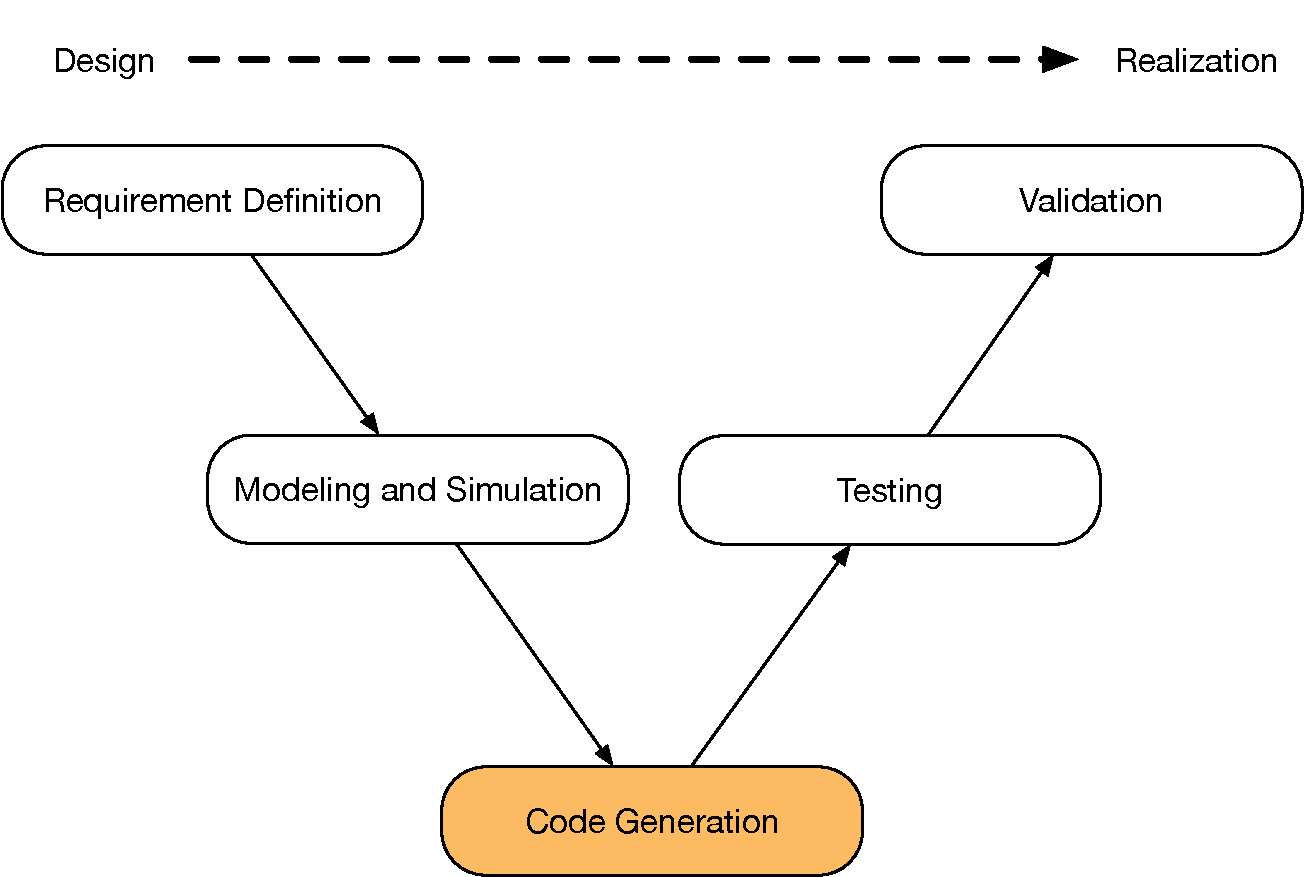
\includegraphics[width=0.7\textwidth]{MBDflowchart}
  \caption{Model-Based Design Flow Chart}
  \label{fig:mbdflowchart}
\end{figure}

\paragraph{} The model includes every component relevant to system behavior-algorithms, control logic, physical components and intellectual property (IP). This make MBD the perfect candidate for a complete work-flow that goes from the system development, verification, validation and deployment. A typical design flow in MDB is shown in figure \ref{fig:mbdflowchart}. The traditional embedded system development process follows the standard \emph{V-shaped} lifecycle. V-cycle splits the product development process into a design and an integration phase. The Code Generation step is the turning point of the process. This work focus on this step. 

%********************************** % Section  **************************************
\section{EMC\textsuperscript{2}}
This work fits inside the European EMC\textsuperscript{2} - "Embedded Multi-Core Systems for Mixed Criticality applications in dynamic and changeable real-time environments" project \cite{emc2artemis}. The objective of the project is to foster changes through an innovative and sustainable service-oriented architecture approach for mixed-criticality applications; the project bundles the power of 98 partners from 19 European Countries and 100 millions of euro in budget.

\paragraph{} Within the EMC\textsuperscript{2} project the objective was to demonstrate the possibility of using a Model-Based Design approach to assist the design and the implementation of mix-critical applications running in multi-core platforms. For that purpose, we selected a typical aerospace use case: motor drive control. This is a widely known application that is used for example in the control of the actuators for the primary and secondary flight control. The platform selected to implement this use case was the Xilinx ZedBoard\texttrademark \cite{zedboard} based on the Xilinx Zynq\textregistered-7000 All Programmable System-on-Chip (SoC). The board is equipped with dual-core ARM\textregistered Cortex-A9 processors and an Artix-7 FPGA which adds more complexity to the design and more flexibility. For the motor control we used the \emph{FMCMOTCON2} \cite{FMCMOTCON2} evaluation kit from Analog Devices (figure \ref{fig:fmcmotcon} which provide a complete motor drive system including a stepper motor, a control board, a low voltage drive board and a Dynamometer drive system.

\begin{figure}[htbp]
  \centering
  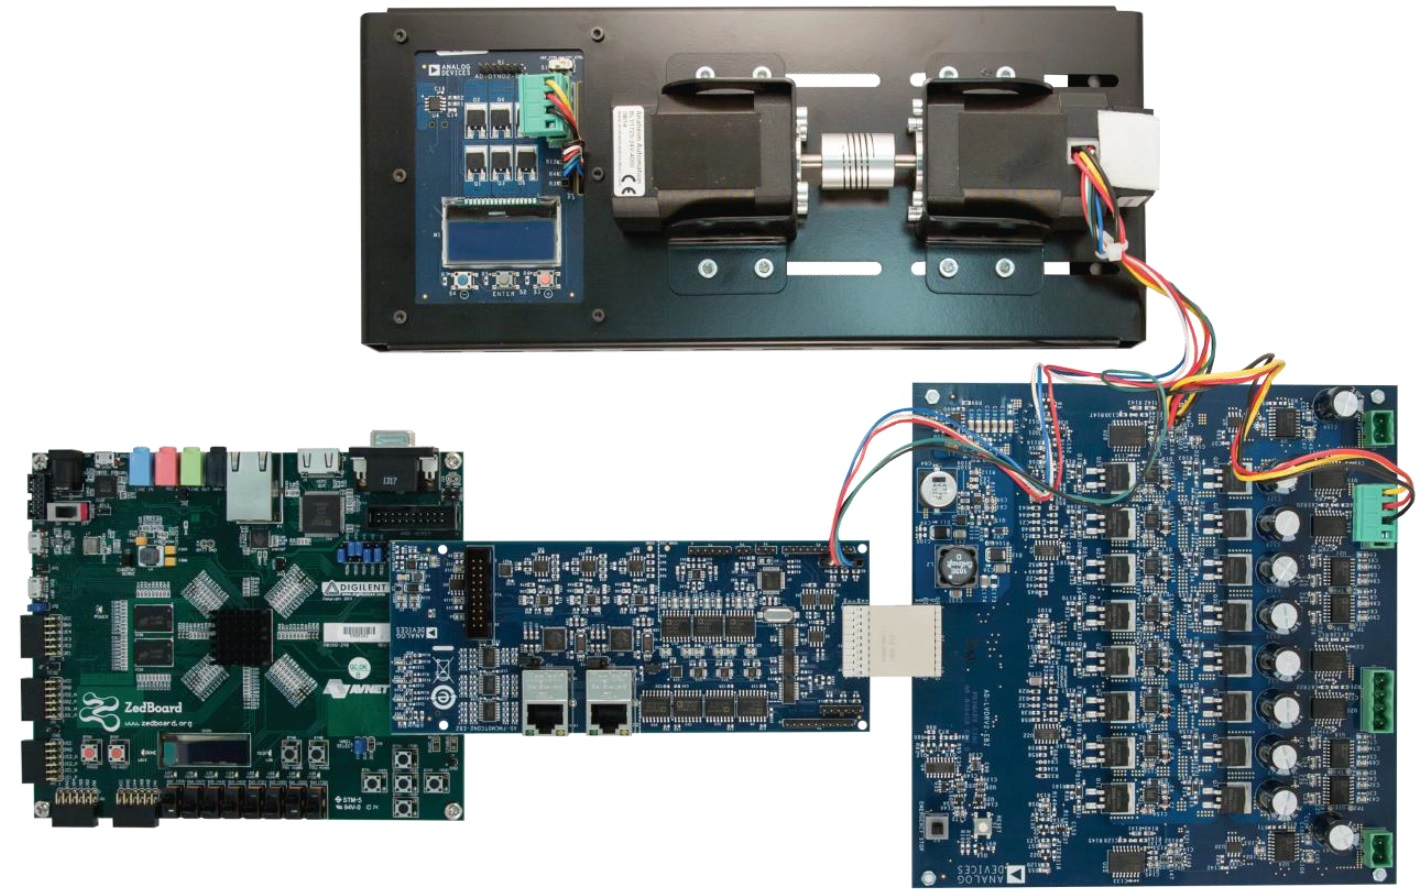
\includegraphics[width=0.9\textwidth]{FMCMOTCON2}
  \caption{Analog Devices FMCMOTCON2 Evaluation Kit}
  \label{fig:fmcmotcon}
\end{figure}

%********************************** % Section  **************************************
%\section{Goal}
%This work presents a model-based approach for automatic code generation for mixed-criticality, multicore, embedded application using an Hypervisor operative system; mainly focusing on aerospace use-cases.
%Our work aims to exploit the multicore platform advantages as much as possible while ensuring an acceptable level of safety among the different mixed critical tasks composing the systems, mainly from aerospace use-cases.
